\chapter{上位机与孪生前端 v2：产品即主角}
\label{ch:host}

v1.2 的孪生前端（gui.html）是一块合格的仪表盘：五支柱、曲线、按钮阵。但 2026-10-02 的用户裁定推翻了它的重心——\textbf{仪表盘只是辅助，数字孪生的核心视图是产品本身及其爆炸视图上的气流、电流走向}；审美对标 Apple 官网的 Liquid Glass~\cite{AppleLiquidGlass}。这不是美术需求，而是产品判断：白牌客户打开页面第一眼要认出"这是一台能买走的机器"，数据长在机器上才有说服力。本章讲 v2 重构（设计规格书 \texttt{2026-10-02-twin-frontend-v2-design.md}）：布局倒转的信息架构、与 PCB 同源的流拓扑、驱动一切电流气流的板级孪生 \texttt{board\_model.py}——包括一次"关断续流 $\tau$ 修正"的审查故事，以及仿真实验室浮层。

\section{布局倒转：从仪表盘到舞台}
\label{sec:host-layout}

v2 的信息架构是一次彻底倒转（图~\ref{fig:v2-intro}）：旧版"图表居中、3D 缩在角落"，新版\textbf{全屏 3D 产品场景是唯一主角}，仪表功能全部退居边缘——顶栏细玻璃条（产品名 + 模式徽章"孪生/真机 BLE" + 连接按钮）；左缘抽屉"控制"（8 阀 + 泵的 Apple 风分段控件）；右缘抽屉"遥测"（默认收起的 sparkline 小卡）；底部中央玻璃胶囊"运输条"（播放/暂停/单步/速度/录制/爆炸滑杆）；最底一行状态（stale 徽章、未标定黄徽、时间与录制状态、仿真实验室入口）。

\begin{figure}[htbp]
  \centering
  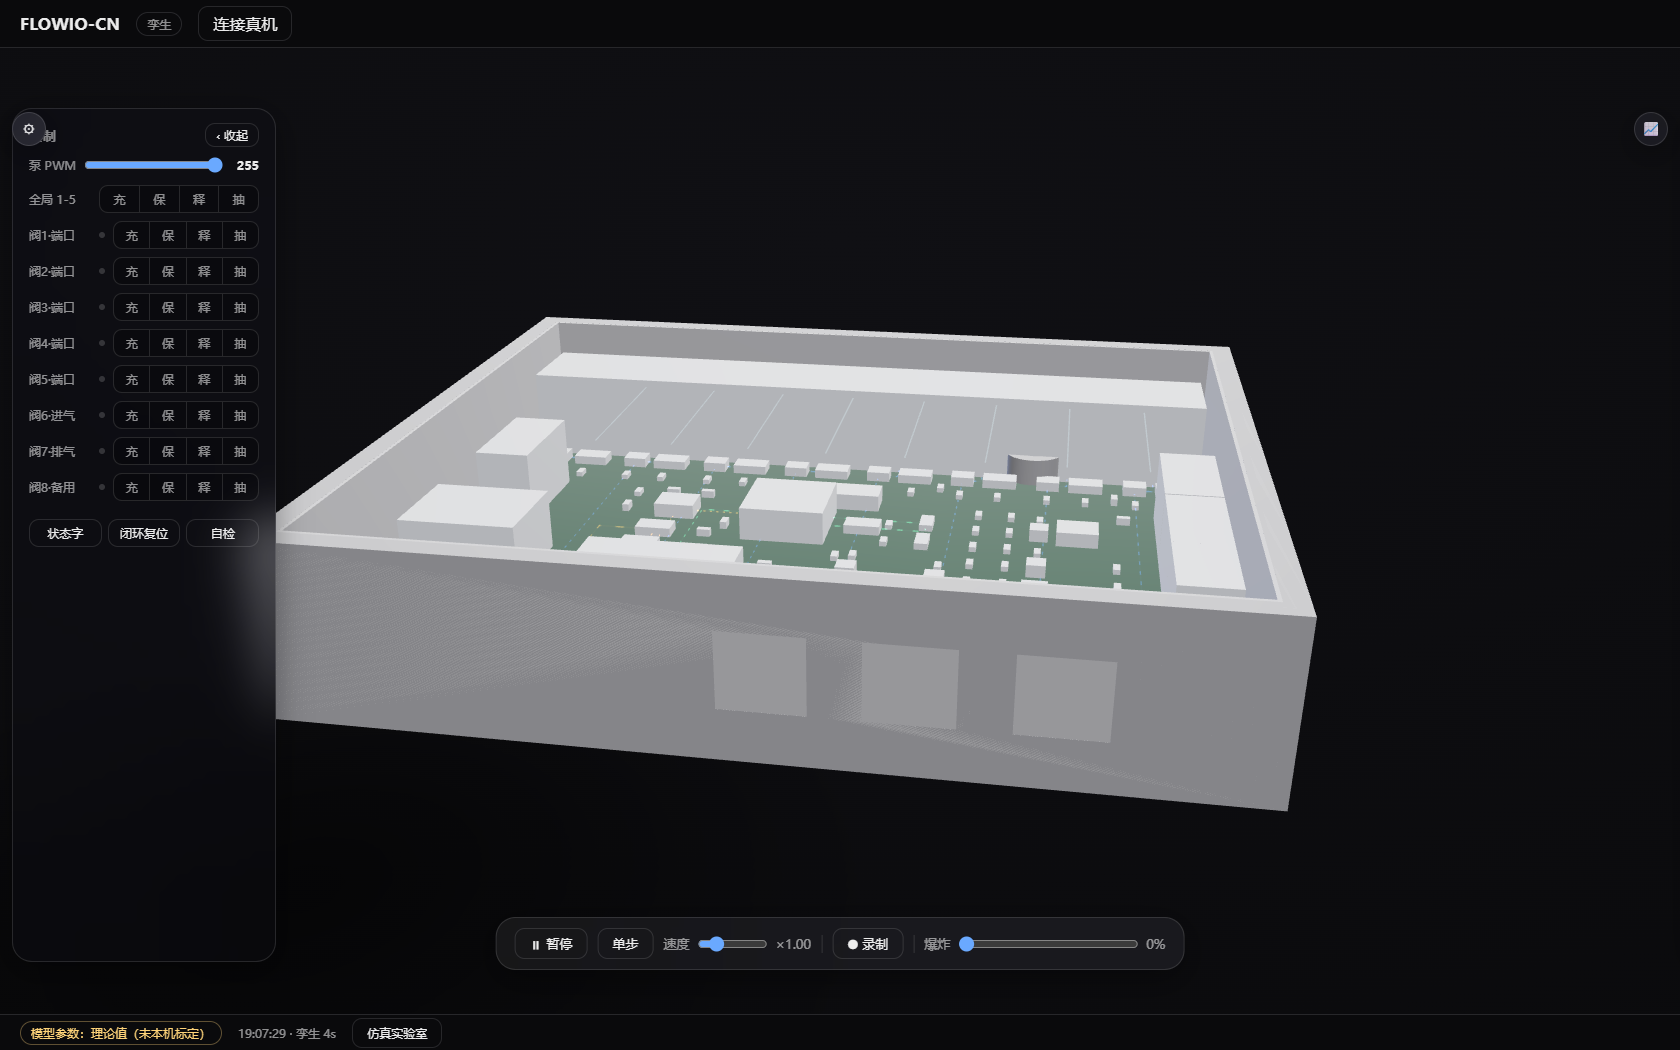
\includegraphics[width=0.95\textwidth]{figures/v2_01_intro.png}
  \caption{v2 首屏：全屏 3D 产品场景 + 左控制抽屉 + 底部运输条玻璃胶囊；状态行常驻"模型参数：理论值（未本机标定）"黄徽章}\label{fig:v2-intro}
\end{figure}

首屏被规定为\textbf{装配叙事}：五部件（上壳/器件阵/PCB/下壳等）从四散位飞入合体，约 1.5\,s（v2 设计令牌规划全局缓动为 \texttt{cubic-bezier(0.22,1,0.36,1)} 的"出舱"手感，实现装配动画取同族 easeOutQuint）；合体后轻微呼吸悬浮（振幅 0.3\,mm、低频呼吸，周期约 25\,s）宣告"这是活的"（慢呼吸节奏避免与数据阅读争夺注意力——动画服务于沉浸而非炫技）。爆炸视图不再是一个按钮，而是运输条里的大滑杆 + "展开/合拢"电影模式（2\,s 往返缓动），语义与第~\ref{ch:enclosure} 章 S3 网格管线的 \texttt{explode*k} 同源。视觉系统的设计令牌写成表（玻璃面板 \texttt{rgba(255,255,255,.06)} + \texttt{backdrop-filter: blur(24px) saturate(180\%)} + 1\,px 半透明边 + 20\,px 圆角；主文本透明度 .92 / 次文本 .55；强调色只有两档——交互电蓝 \#6aa9ff 与流路信号色），并立了三条\textbf{克制红线}：一屏主色不超过两档；禁止网格状仪表盘布局；曲线图去网格线只留细轴线。数字一律等宽（\texttt{tabular-nums}），遥测刷新时数字不跳动。

工程形态坚持\textbf{零构建}：纯 ES Modules，无 React/Vite，\texttt{server.py} 直服（\texttt{/} $\to$ \texttt{webapp/index.html}，\texttt{/webapp/*} 静态资源，\texttt{/classic} 保留旧 gui 一个过渡版本）。七个小模块各司其职：\texttt{main.js} 应用壳（纯对象 store + 订阅）、\texttt{scene.js} 装配/爆炸/材质、\texttt{flows.js} 流光与粒子、\texttt{telemetry.js} 双源轮询、\texttt{panels.js} 抽屉与热点卡、\texttt{simlab.js} 仿真浮层、\texttt{ble.js} 真机模式（第~\ref{ch:ble} 章）。Three.js 从 r128 升 r16x（vendor 单次下载），ECharts 按需加载只供展开小图。这套前端分层并非无源之水：FlowIO 官方软件栈的七层抽象~\cite{flowio-docs-stack}与本孪生实现的逐层对照收录在其官方文档集（\texttt{flowio-softrobotics-docs/}，十九篇）——固件与命令层由第~\ref{ch:firmware} 章的 \texttt{pn\_core} 与 0xA5 协议兑现，Web GUI 层即本章的 v2 前端。

\section{流拓扑同源：make\_flows.py 与 flows.json}
\label{sec:host-flows}

"电流长在产品上"的第一道关卡是\textbf{路径不能手画}——手画的路径与 PCB 对不上，专业客户一眼看穿。v2 的做法是把流拓扑变成网格管线（第~\ref{ch:enclosure} 章）的旁路：\texttt{make\_flows.py} 读 \texttt{fab/flowio-p1-pos.csv} 器件坐标 + 引脚表拓扑，生成 \texttt{flows.json} 与 \texttt{hotspots.json}。坐标系与 S3 的 \texttt{make\_meshes.py} 完全一致（壳坐标：$x=\text{PosX}+2.9$、$y=-\text{PosY}+2.9$、顶面器件 $z=4.0$\,mm），器件焊盘间用曼哈顿折线模拟走线感。防手滑是硬的：任一 ref 在 pos.csv 查不到就报错列出全部缺失，\textbf{不许静默跳过}；hotspots 断言顶面器件；验收测试再断言每条电路路径起止点 = 器件坐标 $\pm0.1$\,mm。

产出的 \texttt{flows.json} 是纯数据：12 条电路路径（DC/USB 双输入 $\to$ SS34 $\to$ 5V 轨 $\to$ buck $\to$ 3V3 轨，加 8 条栅极支路 \texttt{U1$\to$R39..$\to$Q3..$\to$J10..}）+ 8 条气流弧线（各端子出发的二次贝塞尔，端子外延 25\,mm——初版 9\,mm 假设在目视检查中被否决废弃）。每条路径带 \texttt{live} 字段——遥测数据的取值路径：

\begin{lstlisting}[basicstyle=\small\ttfamily, breaklines=true,
  caption={flows.json 的电路与气流条目（摘录）}]
{"id": "gate1", "color": "#6aa9ff",
 "points": [[30.9,19.4,4.0], [7.0,19.4,4.0], [7.0,63.4,4.0], ...],
 "desc": "ESP32→栅极电阻→MOSFET→端子 1",
 "live": "valves[0].i_A", "refs": ["U1","R39","Q3","J10"]}

{"id": "port1", "ref": "J10", "curve": "quadratic",
 "start": [9.4,71.4,4.0], "ctrl": [9.4,85.4,4.0], "end": [9.4,96.4,4.0],
 "desc": "端子→执行器", "live": "valve_duty[1]"}
\end{lstlisting}

\section{电流辉光与气流粒子：数据怎么"长"上去}
\label{sec:host-render}

\texttt{flows.js} 的渲染分两套。\textbf{电流}是 \texttt{THREE.Line} + 自定义 shader 的行进虚线：片段着色器以 \texttt{fract(vT*40 - uTime*uSpeed)} 生成虚线亮带，透明度 $\alpha=(0.08+\text{dash}\times0.92)\times uGain$，叠加混合出辉光。驱动它的就是 live 值的归一——栅极支路 \texttt{valves[n].i\_A/0.36}、电源路径 \texttt{load\_a/3.0}：

\begin{lstlisting}[language=Java, basicstyle=\small\ttfamily, breaklines=true,
  caption={flows.js 的增益与速度映射（摘自源码）：uGain 随电流、uSpeed 随负载}]
const gain = st.connected ? 0.25 + 0.75 * L.live01 : 0.08;   // 断连=8%底光
L.uniforms.uGain.value += (gain - L.uniforms.uGain.value) * Math.min(1, dt * 6);
L.uniforms.uTime.value  = t;
L.uniforms.uSpeed.value = 0.6 + 2.2 * L.live01;              // 满载流速x4.7
\end{lstlisting}

即增益 $uGain \in [0.25, 1.0]$ 随归一电流线性、流速随负载再加速——零负载是静止微光，满载是快速强光，阀一开其栅极支路当拍"通电动起来"（图~\ref{fig:v2-inflate}）。增益用指数平滑过渡（\texttt{dt*6}），遥测的 200\,ms 台阶被抹成连续呼吸，不闪跳。

\begin{figure}[htbp]
  \centering
  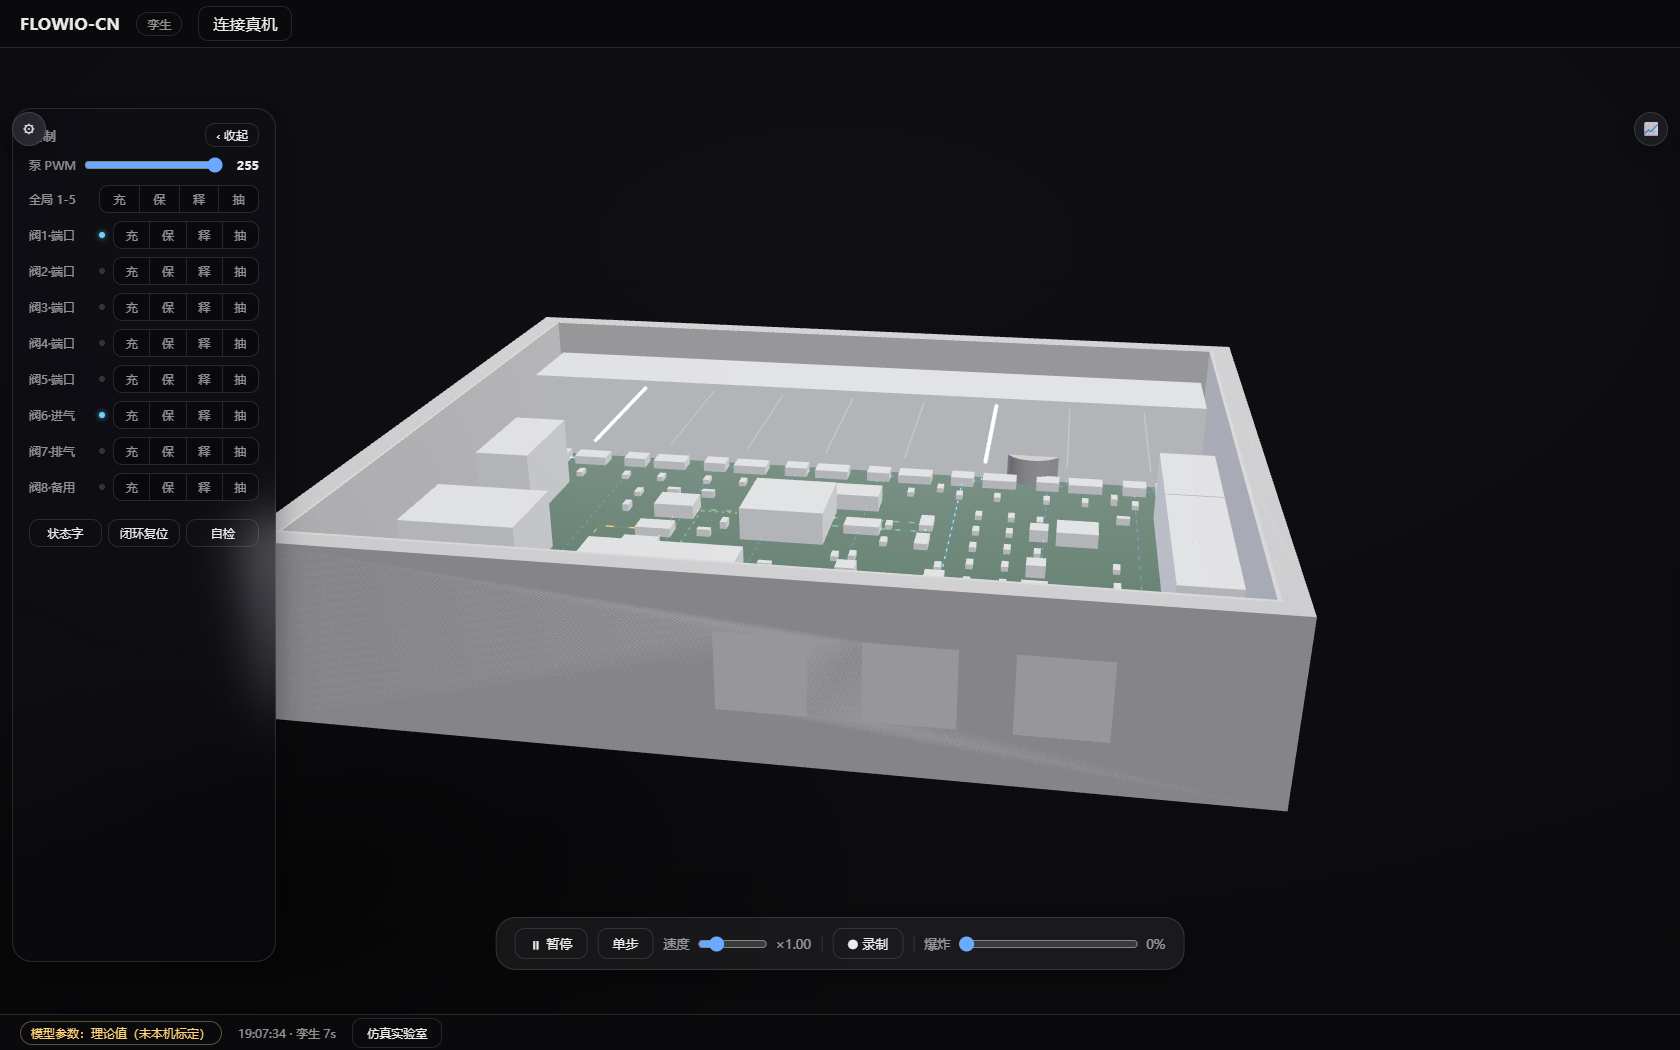
\includegraphics[width=0.95\textwidth]{figures/v2_03_inflate.png}
  \caption{充气态（\texttt{I} 全充）：栅极支路电流辉光 + 端口气流粒子喷出；遥测抽屉/热点卡给出实时值}\label{fig:v2-inflate}
\end{figure}

\textbf{气流}是粒子系统：每端口 50 粒沿贝塞尔曲线参数 $t$ 循环推进（8 端口共 400 粒，守住 $\le500$ 的性能预算），透明度与速度都 $\propto$ PWM duty。两处物理映射值得记：其一，\textbf{方向反转于真空}——\texttt{update()} 里取 \texttt{ports\_p} 中第一个绝对值超阈值的压力符号，负压时速度取负（$t$ 递减，粒子回流）、颜色从正压青 \#6ad4ff 切到真空琥珀 \#ffb454（图~\ref{fig:v2-vacuum}，与第~\ref{ch:acceptance} 章 A102 的差分截图同源）；其二，\textbf{爆炸跟随}——流组的每帧位移直接复制 PCB 部件位移（端子属于 PCB），爆炸滑杆拉开时流线端点随部件平移拉伸，形成"连线不断"的爆炸图观感。静止端口留 8\% 底光提示通道存在；断连时全部回落底光，粒子淡出——安静，不弹窗。

\begin{figure}[htbp]
  \centering
  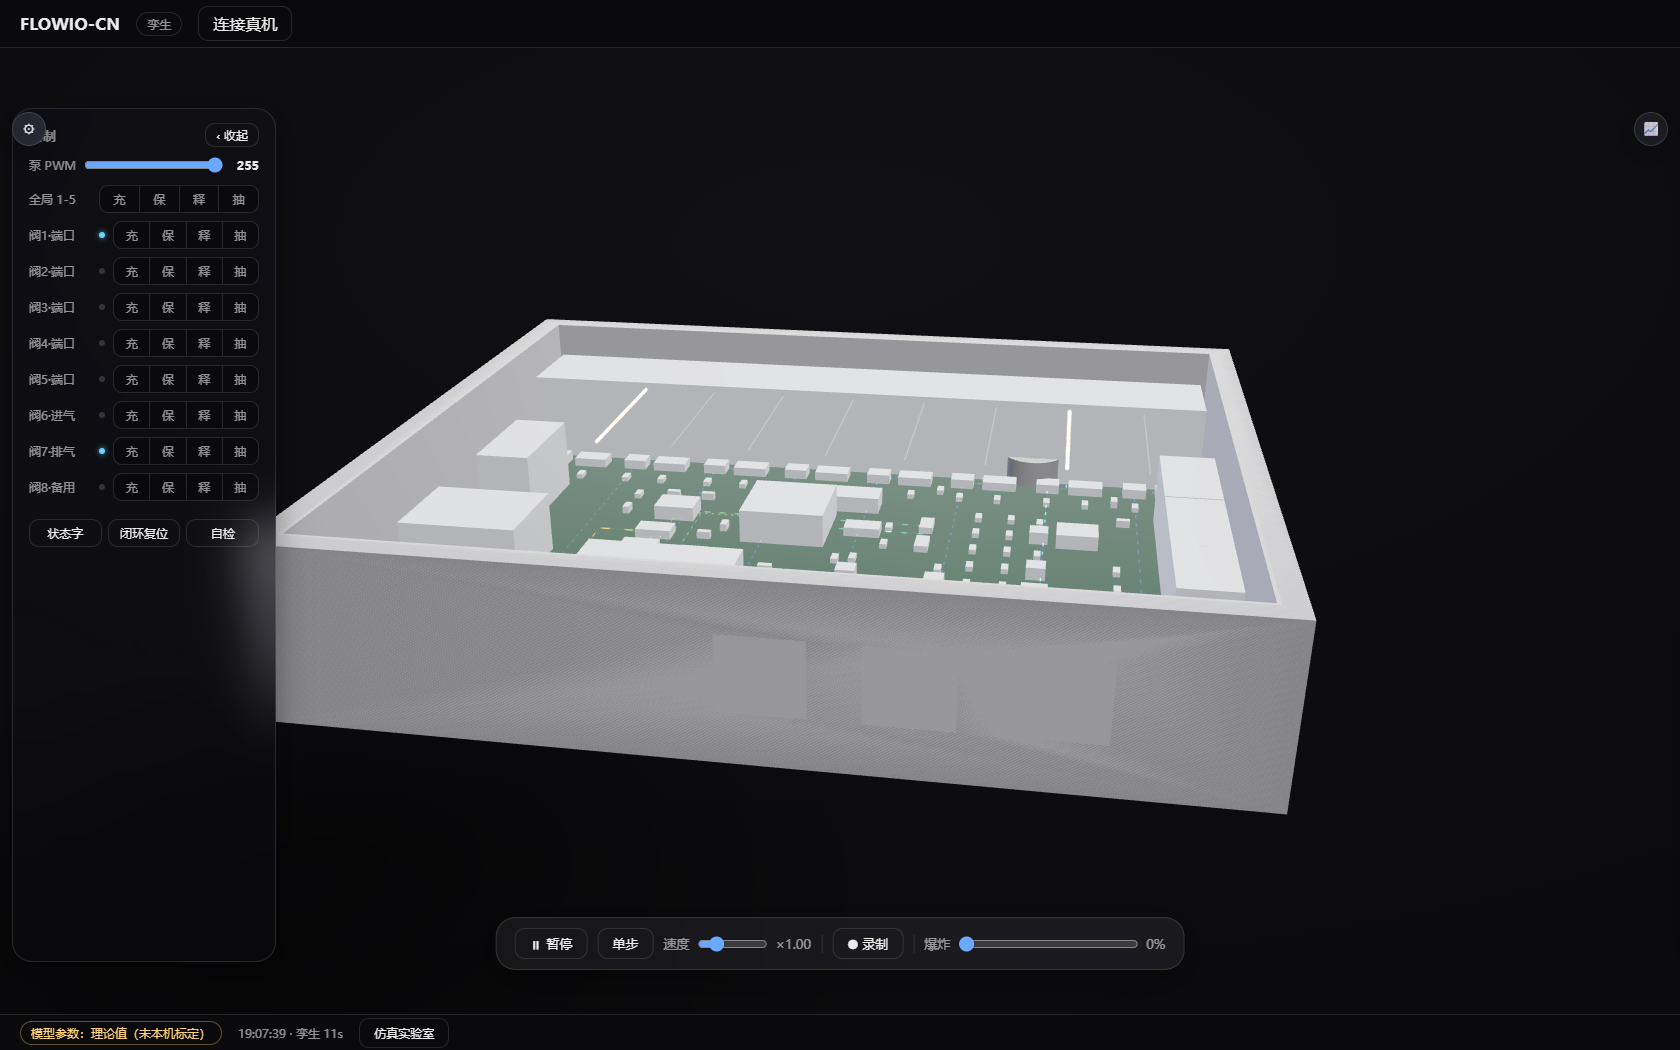
\includegraphics[width=0.95\textwidth]{figures/v2_05_vacuum.png}
  \caption{抽真空态（\texttt{V}）：气流方向反转、颜色转琥珀，压力示数转负——方向与颜色由压力符号驱动}\label{fig:v2-vacuum}
\end{figure}

\textbf{热点卡}补上"点按看器件"的闭环：Raycaster 点击器件（部件级复用 S3；器件级用 \texttt{hotspots.json} 的 ref $\to$ 盒体表），右下滑入玻璃卡显示 2--4 个实时值（如 buck：输出电压/效率/结温；阀道：电流/功率）——\texttt{live} 字段路径直接指向 \texttt{/api/board/state} 遥测（\texttt{board\_model.py} 的契约），点击即取，无需新接口。

\section{板级孪生：解析式 RL 与一次续流 $\tau$ 审查}
\label{sec:host-board}

所有电流辉光的数值都来自 \texttt{board\_model.py}（第~\ref{ch:twin} 章 \S\ref{sec:twin-board} 讲过它的参数成色管理）。这里讲它的另一面：\textbf{作为前端数据源的模型，如何保证算出来的数与电路仿真同物理}——一段真实的审查故事。

阀线圈电流用一阶 RL \textbf{解析式}而非数值积分。开通侧直接：
$\tau_\text{on}=L/(r_\text{coil}+r_\text{ds})\approx1.78$\,ms，$i = I_\infty + (i_0 - I_\infty)e^{-t/\tau_\text{on}}$，稳态 $I_\infty=5\,\text{V}/14.04\,\Omega\approx0.356$\,A——100\,ms 步长下 $dt/\tau\approx56$，电流完全建立，解析式既准又免积分。

关断侧最初（实施计划草案）写成开通的镜像：衰减到 0，$\tau$ 沿用 $L/(r_\text{coil}+r_\text{ds})$。\textbf{审查纠正了它}：MOS 已断开，线圈电流走的是 SS14 续流回路，回路里没有 $r_\text{ds}$、只有线圈电阻与二极管钳位电压——正确模型是

\begin{lstlisting}[language=Python, basicstyle=\small\ttfamily, breaklines=true,
  caption={board\_model.py 的关断续流（节选自源码，开通稳态行与循环头从略）：$\tau$ 换回路，负稳态 + 过零钳位}]
tau_on  = p["l_coil"] / (p["r_coil"] + p["rds"])   # 激励回路: L/(r_coil+rds)
tau_off = p["l_coil"] / p["r_coil"]                # 续流回路: L/r_coil (SS14 钳位)
i_inf_off = -p["vf_fw"] / p["r_coil"]              # 续流负稳态 (过零截止)
...
if on:
    self.i[k] = i_inf + (i0 - i_inf) * math.exp(-dt / tau_on)
else:
    i = i_inf_off + (i0 - i_inf_off) * math.exp(-dt / tau_off)
    self.i[k] = i if i > 0.0 else 0.0              # 二极管反向截止钳位
\end{lstlisting}

差别看似细微（$\tau_\text{off}=1.79$\,ms 与 $\tau_\text{on}=1.78$\,ms 几乎同值），\textbf{形状}却不同：续流回路的目标值是负稳态 $-V_F/r_\text{coil}$，电流以更陡的斜率冲向零并在约 4.9\,ms 处被二极管反向截止钳在零——镜像指数衰减则拖着渐近尾巴永不归零。哪个对？续流二极管存在就不容商量。测试把它钉死：\texttt{test\_board\_model.py} 断言关阀 10\,ms 后电流已钳 0（$0\le i<0.35\times0.5$）。注释同时声明防线的另一半：\texttt{vf\_fw=0.35} 与 \texttt{sim\_engine} 续流 ODE 的 \texttt{VF\_FW} 同源——\textbf{两个实现解同一个物理量，必须共享同一组常数}，否则板级模型与电路仿真各漂各的，前端热点卡与仿真实验室对不上数，孪生就自己拆自己的台。

同一审查还抓出两处"双源漂移"。\textbf{其一}，\texttt{telemetry()} 快照曾直接返回 buck 标称输出 3.269\,V，而历史曲线按负载调整率公式算出 3.2638\,V——同一页面上"当前值"与"曲线末端"差 5\,mV。修正：快照与 \texttt{step()} 用\textbf{同一式子}重算（$v_{33}=v_\text{out}-r_\text{load}\cdot I_\text{logic}$），标称值另存 \texttt{v\_nom} 字段。\textbf{其二}，buck 效率与损耗曾是 @3\,A 工况的常量快照（\{706,162,436,85\}\,mW），与实时负载无关；修正为 CCM 损耗分解动态计算（开关/绕线/二极管/开关损耗四项，公式与 \texttt{sim\_engine.\_buck} 同源），$v_5$ 跌 $\to$ 占空比 $D$ 升 $\to$ 损耗随之变化，测试断言空载与满载的损耗向量\textbf{不相等}。三条修正合起来是一个方法论：\textbf{凡是同一物理量有两个公式，就让它们同源；凡是同源，就用测试钉住}。

\section{双源轮询与安静降级}
\label{sec:host-telemetry}

数据管道 \texttt{telemetry.js} 以 200\,ms 节拍\textbf{交替}轮询两个源：偶拍 \texttt{/api/board/state?since=}（电气遥测 + 增量历史，\texttt{since} 游标去重边界点）、奇拍 \texttt{/api/state}（气动：阀 duty/压力/状态字）。结果双管道分发：\texttt{setState} 进 store（抽屉 sparkline 消费）、\texttt{flows.update} 进流光（粒子消费）。前端自持两级缓冲——\texttt{hist} 是服务端权威历史的镜像（v5/v33/load，60 点 sparkline 窗口 $\approx$24\,s，展开小图 600 点 $\approx$4\,min），\texttt{snap} 是无服务端历史的快照环（三结温最大值、效率）。停轮询的三种条件：页面隐藏、孪生时间暂停、\textbf{BLE 真机接管}（\texttt{store.bleActive}，第~\ref{ch:ble} 章）；连续两次失败才置 \texttt{stale}（单次抖动不算），stale 后主场景流光淡出为底光、状态行亮"遥测冻结"徽章——不弹窗，不渲染过期值。

\section{仿真实验室：四电路重算浮层}
\label{sec:host-simlab}

仿真实验室是 v1.2 四电路仿真的 v2 皮肤：从底部升起的全屏玻璃接管浮层，四个分段——Buck 电源（TPS54331 $\to$ 3.3\,V/3A）、双源二极管或（SS34$\times$2）、阀驱动（AO3400A 低边 + RL）、I\textsuperscript{2}C 上拉（TCA9548A 总线 RC）。它不常驻、不抢主场景。后端是 \texttt{sim\_engine.py} 的参数化行为级仿真（无 ngspice 环境下的自研状态机，纯 stdlib）：每电路一张参数域表——参数名、上下限、默认值（默认值与 BOM 一致，如 buck 的 $C_\text{out}$=100+10+3\,$\mu$F 合成 113），越域抛 \texttt{ParamError} 并指名道姓（前端 400 红条提示）；返回指标（带通过/告警判定徽章）与降采样波形数组，前端 canvas 自绘细线 + 细轴线 + 稀疏刻度（\S\ref{sec:host-layout} 的克制红线）。接口复用 v1.2 端点零改动：\texttt{GET /api/board/sim/presets}（参数域表 $\to$ 动态表单）、\texttt{POST /api/board/sim}（重算）。参数域的意义在验收侧有一次实战：I\textsuperscript{2}C 上拉 4.7\,k$\Omega\times$115\,pF 的上升时间实测告警案例，即用该浮层扫参数定位（第~\ref{ch:acceptance} 章工单 A103）。

验收动线与旧版一样是"测试 + 目视"双轨：\texttt{test\_webapp.js} 44 断言换新 DOM 锚点（场景 canvas、抽屉开关、热点卡、sim 浮层、运输条），外加 \texttt{?debug} 浮层的 60\,s fps 采样（预算 $\ge$45）；而装配动画、爆炸跟随流线、阀开栅极亮起、真空回流反向、断连态七项走\textbf{强制目视检查}（截图 + 机内视觉逐项审）——首屏、充气、真空三张图（图~\ref{fig:v2-intro}--\ref{fig:v2-vacuum}）正是 26 项目视记录的直接复用（工单 A101/A102，第~\ref{ch:acceptance} 章）。旧 \texttt{gui.html} 打"经典版"标保留在 \texttt{/classic}（P1 面板独有的泄漏注入/物理注入/scheduler 编排等调试入口迁移完成前不退线），v2 验收通过后再定下线。

\section*{本章小结}
v2 的本质是把孪生前端从"看数据"改成"看产品"：布局倒转让 3D 场景当主角，流拓扑由 \texttt{make\_flows.py} 从 pos.csv 同源生成（不许手画、不许静默跳过），电流辉光的增益与流速、气流粒子的方向与颜色全部由遥测数据驱动，断连与降级一律安静。数值侧的底气来自 \texttt{board\_model.py}：RL 解析式经过关断续流 $\tau$ 的审查修正、快照与历史同式重算、损耗动态化——同一物理量同源、同源被测试钉死。孪生侧至此闭环；下一章给外部开发者一条 5 分钟上手的路：Python SDK。
